
\section{Zakres zastosowań coachingu}

% Jak teraz rozumiem zakres zastosowan coachingu?
% Ktore sposrod standardow etycznych ICF oraz Izby Coachingu uwazam za szczegolnie istotne z wlasnej praktyki zawodowej - uzasadnij z jakich powodow?
% Komu, kiedy i w jakich sytuacjach zaoferowalabym coaching?
% w jakich przypadkach przekazalbym klientowi kontakt do innego (jakiego?) specjalisy?

Zakres możliwych zastosowań coachingu jest niezwykle szeroki, ponieważ może on być stosowany bez względu na wiek, płeć, status społeczny itd.
W życiu każdej osoby wysoce prawdopodobne są sytuacje w których skorzystanie z procesu coachingowego może przynieść owocne rezultaty.
Jednocześnie należy podkreślać, że coaching nie jest lekarstwem na wszystkie problemy i wielu przypadkach nie jest wskazany.
Wiele tego typu dylematów zostało już w przeszłości rozważonych przez organizacje związane z coachingiem co doprowadziło do powstania
standardów etycznych. Niestety prawie każda organizacja definiuje własny standard, co prowadzi do braku standaryzacji. Z drugiej strony
tematyka omawiana przez te standardy jest bardzo podobna, więc zazwyczaj różnice są nieznaczne.

\subsection{Standardy etyczne w pracy coacha}
Bazując na doświadczeniu autora pracy punkt 9. z sekcji 3. Standardu Etycznego Postępowania ICF \cite{kodeksicf} jest szczególnie istotny.
Ta sekcja standardu nosi tytuł \emph{Profesjonalne postępowanie wobec klientów} i porusza różnego rodzaju zagadnienia związane
z uczciwością, szacunkiem i moralnością. Wspomniany wyżej punkt 9. ma następującą treść:
\begin{quote}
\centering
\emph{ "Będę zalecać klientowi korzystanie z usług innych specjalistów, kiedy uznam to za odpowiednie lub konieczne."}
\end{quote}
W obecnej sytuacji wśród osób prywatnych zainteresowanych rozwojem osobistym nadal nie ma dużej czytelności pomiędzy różnymi
możliwymi metodami rozwoju. Osoby dla których bardziej odpowiednia mogłaby być np. terapia, wysyłane są na coaching. Spowodowane
to jest głównie faktem, że coaching jest w tym momencie zyskującym na popularności zjawiskiem. Zdaniem autora pracy dpowiedzialność
za edukowanie klientów o wadach i zaletach oraz formie różnych metod rozwoju osobistego leży w obowiązku każdego coacha.

Sytuację tę komplikuje również gwałtowny wzrost zainteresowania coachingiem. Większość młodych ludzi zetknęła się z
pojęciem \emph{coaching}, ale zaledwie niewielkie grono z nich ma prawidłową wiedzę na temat tego co to pojęcie oznacza.
Wzrost zainteresowania coachingiem na terenie Polski jest przedstawiony na wykresie \ref{wykres}. Można na nim zaobserwować
około czterokrotny wzrost ilości wyszukiwaniach w wyszukiwarce Google fraz związanych z coachingiem w latach 2007-2012,
czyli okresie zaledwie pięciu lat. Jednocześnie widać bardzo szybko malejące zainteresowanie doradztwem, które obecnie plasuje się
na zbliżonym poziomie do coachingu. Wykres umożliwia również zaobserwowanie jak marginalny charakter względem coachingu i
doradztwa mają obecnie takie formy samorozwoju jak mentoring czy counseling.

\begin{figure}[!ht]
  \centering
  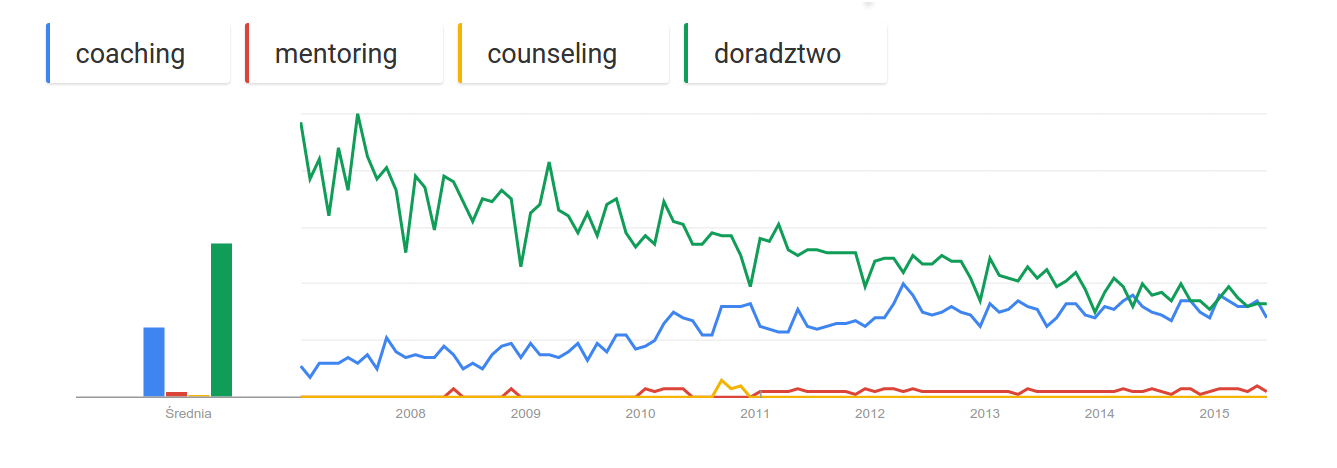
\includegraphics[width=17cm]{img/popularnosc}
  \caption{Popularność metod rozwoju osobistego na podstawie liczby zapytań do wyszukiwarki internetowej Google. Wykres obejmuje przedział czasowy w latach 2007-2015.}
  \label{wykres}
\end{figure}

Drugim szczególnie istotnym punktem zdaniem autora pracy jest dyskrecja w sprawach dotyczących klienta. Cytując za Kodeksem Etycznym Izby Coachingu \cite{kodeksib}:
\begin{quote}
\centering
\emph{"6.2 Jeśli dobro Klienta wchodzi w konflikt z lojalnością zawodową, Coach pracuje przede wszystkim dla dobra Klienta i postępuje zgodnie z uzgodnionym kontraktem.".}
\end{quote}
Widocznym wnioskiem z tego punktu jest jak niezwykle ważne staje się czytelne ustalanie kontraktu pomiędzy coachem a klientem.
Szczególna uwaga powinna mieć miejsce jeśli w proces zaangażowany jest również zewnętrzny zleceniodawca.

\subsection{Grupa docelowa procesu coachignowego}

\begin{itemize}
  \item im bardziej samodzielnym tym lepiej, ale przynajmniej w obszarze celów procesu
  \item osobom o wysokiej motywacji
  \item znajdującym się w nowej dla nich sytuacji (którym prawdopodobnie towarzyszy wysoka motywacja pozytywna) lub
       ulegających wypaleniu lub frustracji (wysoka motywacja negatywna). W drugim przypadku należy również rozważyć
       mentoring/szkolenia (np. frustracja wynika z braków wiedzy i przez to nie są osiągane efekty) lub consueling.
  \item dla osób stojących przed dylematem i aktywnie szukających jego rozwiązania
\end{itemize}

Tak jak zostało to podkreślone w poprzedniej sekcji - bardzo istotnym aspektem pracy coacha jest wiedza o tym, kiedy klient powinien
zostac skierowany do innego specjalisty. Przy pomocy tabeli \ref{table:kategorie} można zidentyfikować następujące przypadki:
\begin{itemize}
\item[--] W przypadku osoby potrzebującej wiedzy i gotowych rozwiązań - mentoring lub szkolenia.
\item[--] W przypadku osoby o niskiej motywacji / wypaleniu - consueling.
\item[--] W przypadku osób stojących przed decyzją, ale nie dylematem - tzn. potrzebujących wiedzy i oceny sytuacji - pomoc konsultant.
\item[--] W przypadku osób w stanach depresyjnych, nie widzących możliwych rozwiązań i niskiej motywacji do wprowadzania zmian w swoim życiu - terapia.
\end{itemize}
